% TEXINPUTS=.:$HOME/git/bvtex: latexmk  -pdf <main>.tex
\documentclass[xcolor=dvipsnames]{beamer}

\input{defaults}
\input{beamer/preamble}

\setbeamertemplate{navigation symbols}{}
% \setbeamertemplate{background}[grid][step=1cm]

\usepackage{siunitx}
\usepackage{xmpmulti}
\usepackage[export]{adjustbox}

\usepackage[outline]{contour}
\usepackage{tikz}
\usetikzlibrary{shapes.geometric, arrows}
\usetikzlibrary{positioning}

\definecolor{bvtitlecolor}{rgb}{0.98, 0.92, 0.84}
\definecolor{bvoutline}{rgb}{0.1, 0.1, 0.1}

\renewcommand{\bvtitleauthor}{Brett Viren}
\renewcommand{\bvtitle}{\LARGE LARF Status\\{\small 3D Field and Detector Response Calculations}}
\renewcommand{\bvtit}{LARF Status}
\renewcommand{\bvevent}{\Large BNL-$\mu$Boone\\\today}
\renewcommand{\bvbeamerbackground}{}

\newcommand{\microboone}{MicroBooNE\xspace}


\begin{document}
\input{beamer/title.tex}
\input{beamer/toc.tex}
\section{Parallel Wires}



\begin{frame}
  \frametitle{Parallel Wires - Parameters}
  Try to match 2D calculation with 3D, parallel wires.

  \vspace{3mm}

  \begin{description}
  \item[planes] 13 wires in each plane, all parallel.
  \item[wires] 3mm pitch and gap, 0.15mm radius, \\30mm length, 1.5mm meshing.
  \item[cathode] -500 V (and ground) planes at +20 mm (-20 mm), 2.5mm meshing.
  \item[precision] Double the BEM Gaussian quadrature orders.
  \item[resolution] raster grid at 500x10x500.
  \end{description}
\end{frame}

\begin{frame}
  \begin{columns}
    \begin{column}{0.5\textwidth}
      \begin{center}
        \includegraphics[width=\textwidth]{twodee-fine-x.pdf}

        \includegraphics[width=0.7\textwidth]{twodee-fine-z.pdf}
      \end{center}
    \end{column}
    \begin{column}{0.5\textwidth}
      \begin{center}
        \includegraphics[width=\textwidth]{twodee-fine-iso.pdf}

        \includegraphics[width=0.7\textwidth]{twodee-fine-y.pdf}
      \end{center}
    \end{column}
  \end{columns}
\end{frame}


\begin{frame}
  \frametitle{Parallel Wires - Slice Through Weighting Potentials}
  \begin{columns}
    \begin{column}{0.3\textwidth}
      \begin{center}
        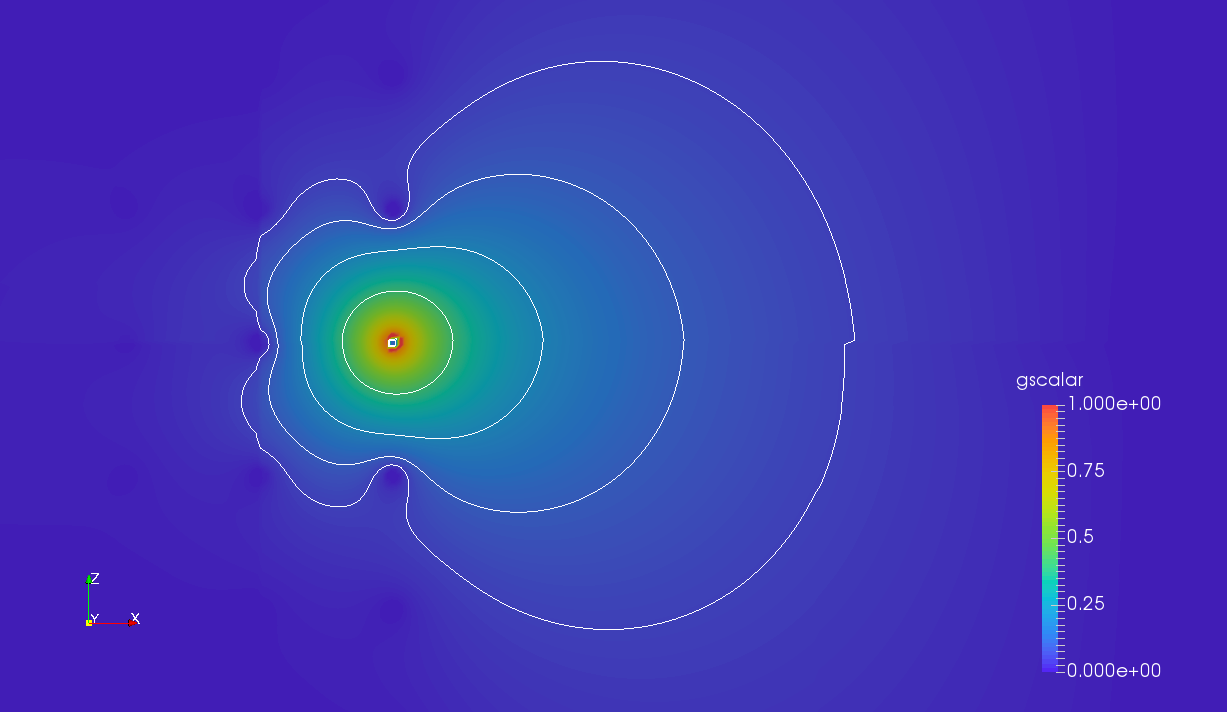
\includegraphics[height=2cm]{twodee-fine-u7.png}

        \scriptsize U plane
      \end{center}
    \end{column}
    \begin{column}{0.3\textwidth}
      \begin{center}
        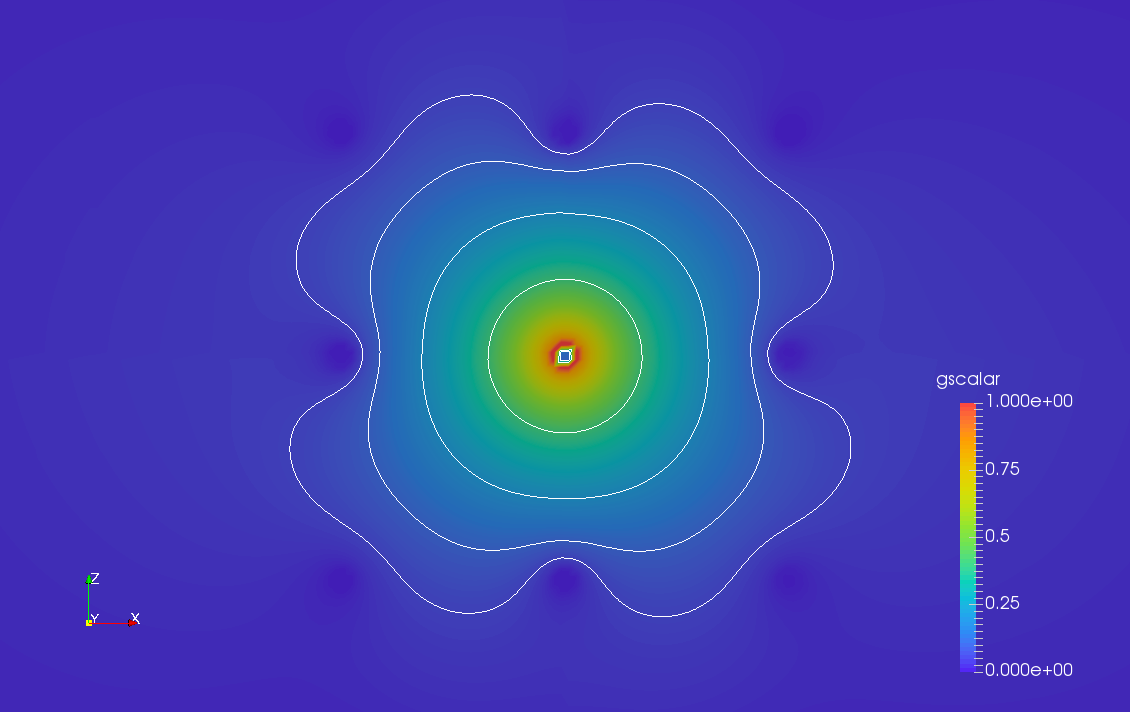
\includegraphics[height=2cm]{twodee-fine-v7.png}
        
        \scriptsize V plane
      \end{center}
    \end{column}
    \begin{column}{0.3\textwidth}
      \begin{center}
        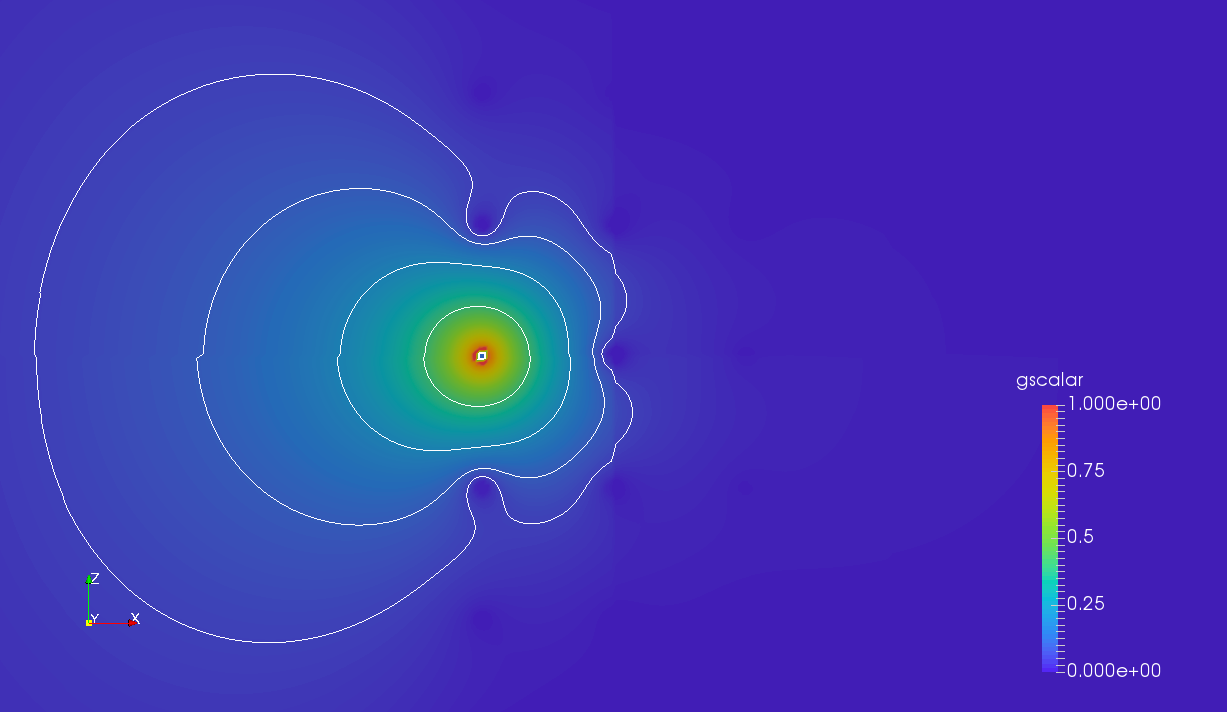
\includegraphics[height=2cm]{twodee-fine-w7.png}

        \scriptsize W plane
      \end{center}
    \end{column}
  \end{columns}

  \begin{itemize}\footnotesize
  \item X-Z slice through plane of symmetry (Y=0).
  \item Color shows weighting potential: 0-100\%.
  \item Lines: 5\%, 10\%, 20\%, 40\% weights.
  \item Gaussian quadrature imprecision visible in some jaggy contous lines.
  \item Small spatial fluctuations near wires, but somewhat obscured.
    \begin{itemize}\scriptsize
    \item Note: inside wire is $\sim$0V, square shape is pixelization.
    \end{itemize}
  \end{itemize}

  \begin{center}
    Visual comparison with Bo's 2D fields show good agreement.

    For now, consider this enough validation to move forward.
  \end{center}
\end{frame}

\begin{frame}
  \frametitle{Parallel Wires - Steps}
  \begin{center}
    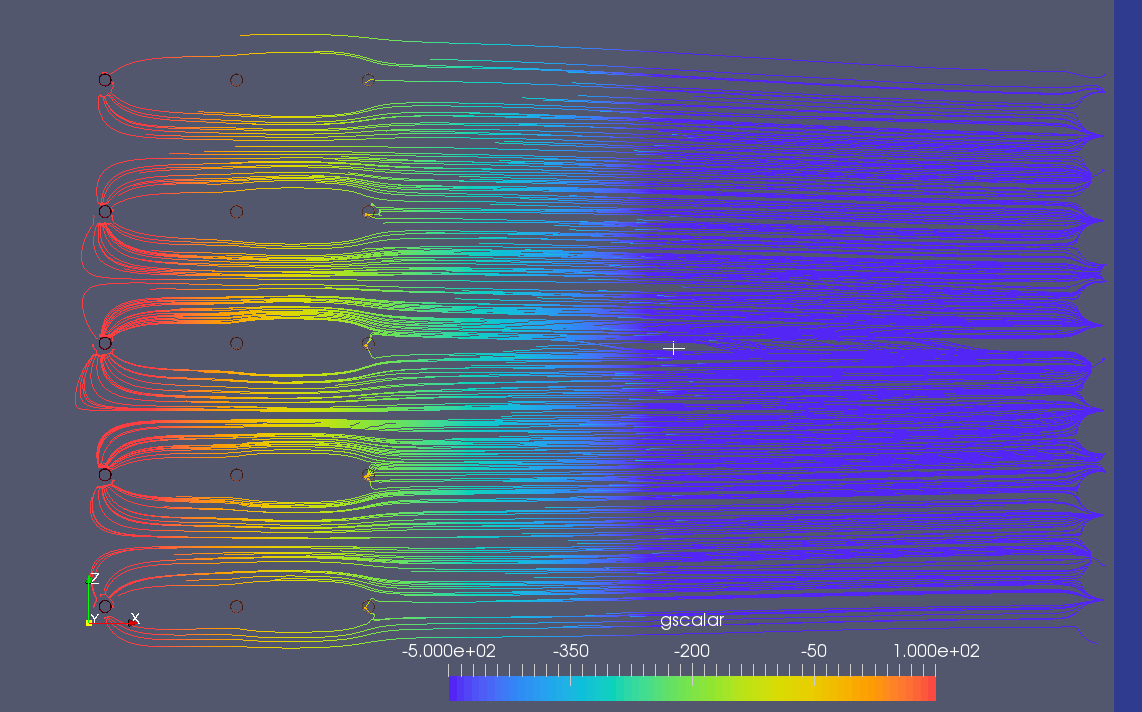
\includegraphics[width=0.7\textwidth]{twodee-fine-drift-steps-plan.png}    
  \end{center}
  \begin{itemize}\footnotesize
  \item Uses ParaView's build in R-K stepper, color still shows potential.
  \item This is looking down the Y-axis, but actually 3D steps.
  \item Each stepping goes for fixed length and then quits, tracks
    terminating around the cyan, explained next.
  \end{itemize}
\end{frame}

\begin{frame}
  \frametitle{Parallel Wires - Steps Side Vie...WHOOPS!}
  \begin{center}
    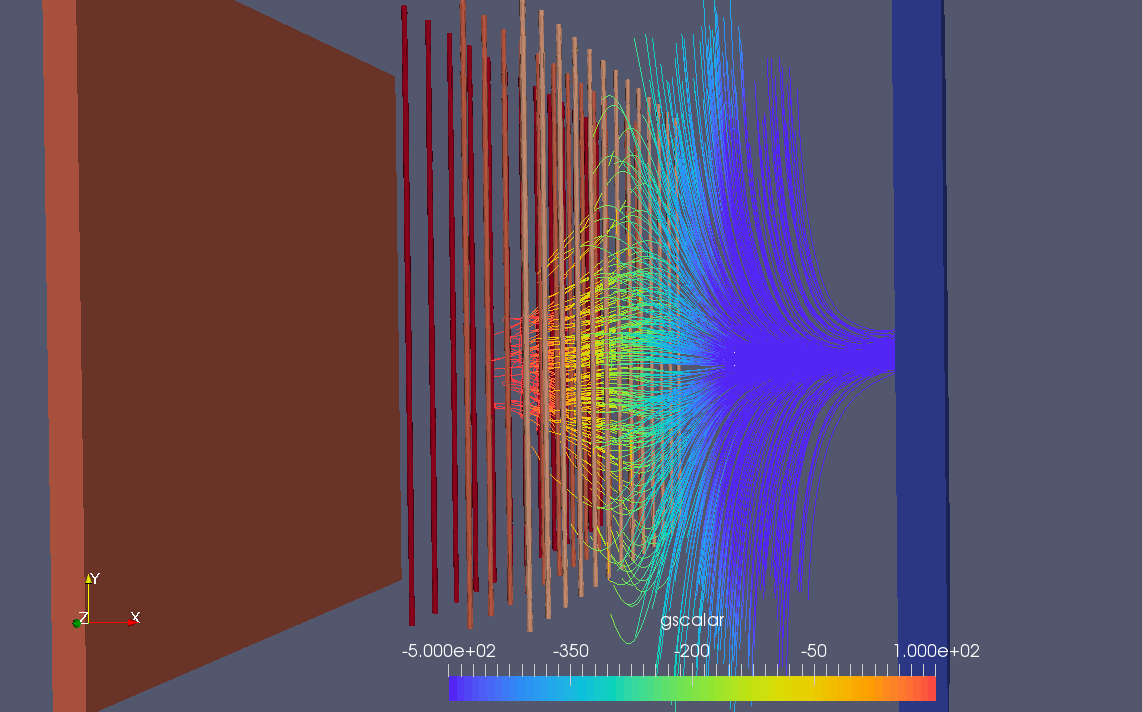
\includegraphics[width=0.7\textwidth]{twodee-fine-drift-steps-side.png}    
  \end{center}
  \begin{itemize}\footnotesize
  \item Side view of same scene.
  \item But, what's with this divergence in the vertical direction?
    \begin{itemize}\scriptsize
    \item[$\rightarrow$] Bug in gradient! I was not respecting voxel dimensions!
    \item[$\rightarrow$] Artificial $50\times$ magnification in vertical derivative.
    \end{itemize}
  \end{itemize}
  ParaView visualization makes bugs like this (painfully) obvious!
\end{frame}

\begin{frame}
  \frametitle{Visualizing Bugs}
  \begin{columns}
    \begin{column}{0.5\textwidth}
      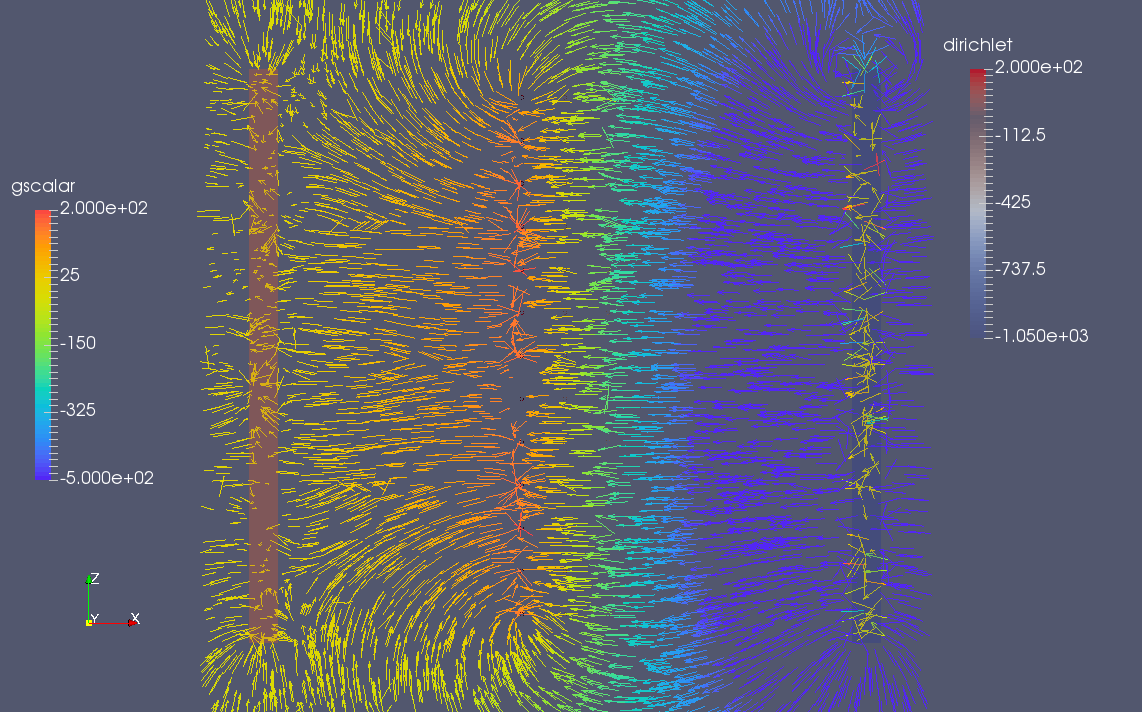
\includegraphics[width=\textwidth]{twodee-fine-arrows-plan.png}      
    \end{column}
    \begin{column}{0.5\textwidth}
      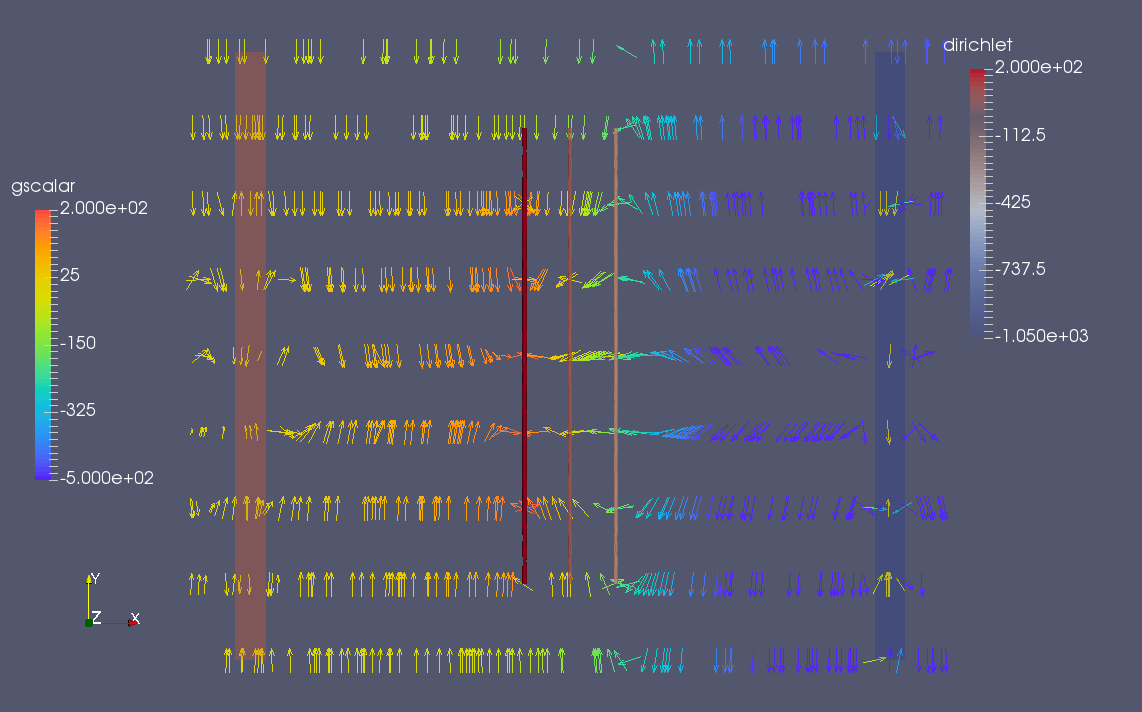
\includegraphics[width=\textwidth]{twodee-fine-arrows-side.png}      
    \end{column}
  \end{columns}
  \footnotesize
  \begin{itemize}
  \item Color of arrows is potential.
  \item X-Z and X-Y slices with vector field drawn as arrows.  
  \item Clearly vector field in Y direction is wrong.
  \item Voxels are 0.1mm in X and Z, 5mm in Y $\Rightarrow 50\times$ mistake.
  \end{itemize}
  Anyway, ParaView is very useful to find dumb bugs.
\end{frame}

\begin{frame}
  \frametitle{After gradient fix - vector field}
  \begin{columns}
    \begin{column}{0.5\textwidth}
      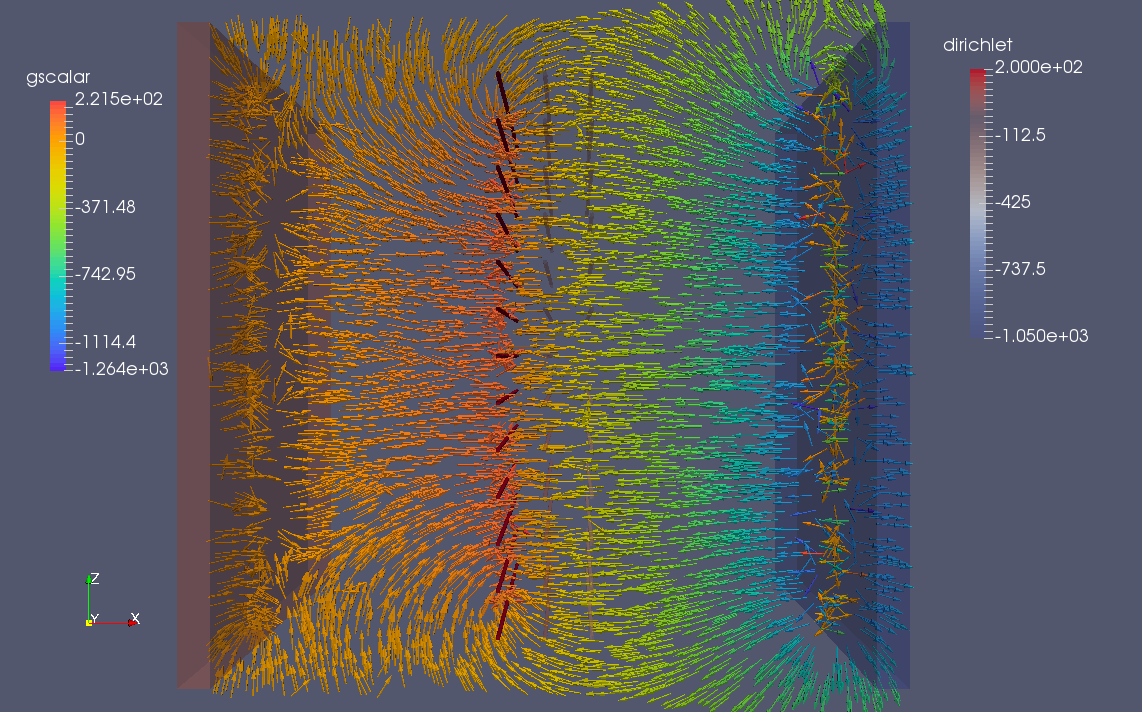
\includegraphics[width=\textwidth]{twodee-fine-arrows-plan-fixgrad.png}      
    \end{column}
    \begin{column}{0.5\textwidth}
      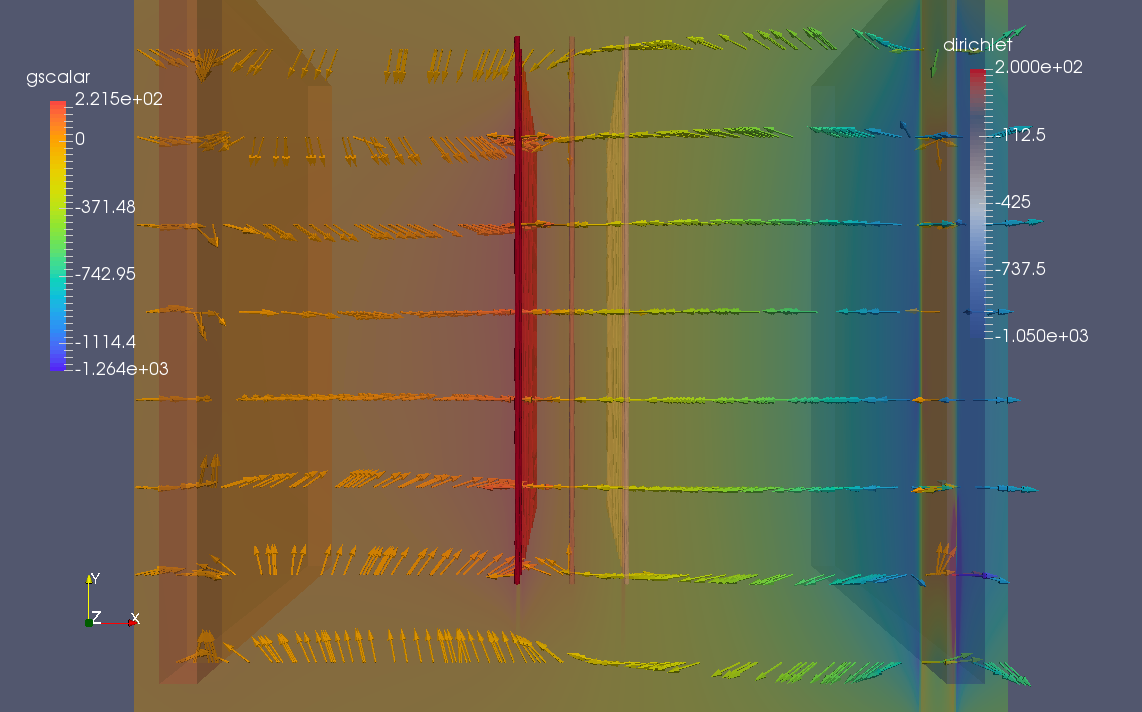
\includegraphics[width=\textwidth]{twodee-fine-arrows-side-fixgrad.png}      
    \end{column}
  \end{columns}
  \footnotesize
  \begin{itemize}
  \item Much more reasonable looking vectors.
  \item Still some divergence toward top/bottom, but it's reasonable.
    \begin{itemize}\scriptsize
    \item This will limit the amount of ``useful'' volume to look at (next topic).
    \end{itemize}
  \end{itemize}
\end{frame}

\begin{frame}
  \frametitle{After gradient fix - Recheck Steps}
  \begin{columns}
    \begin{column}{0.5\textwidth}
      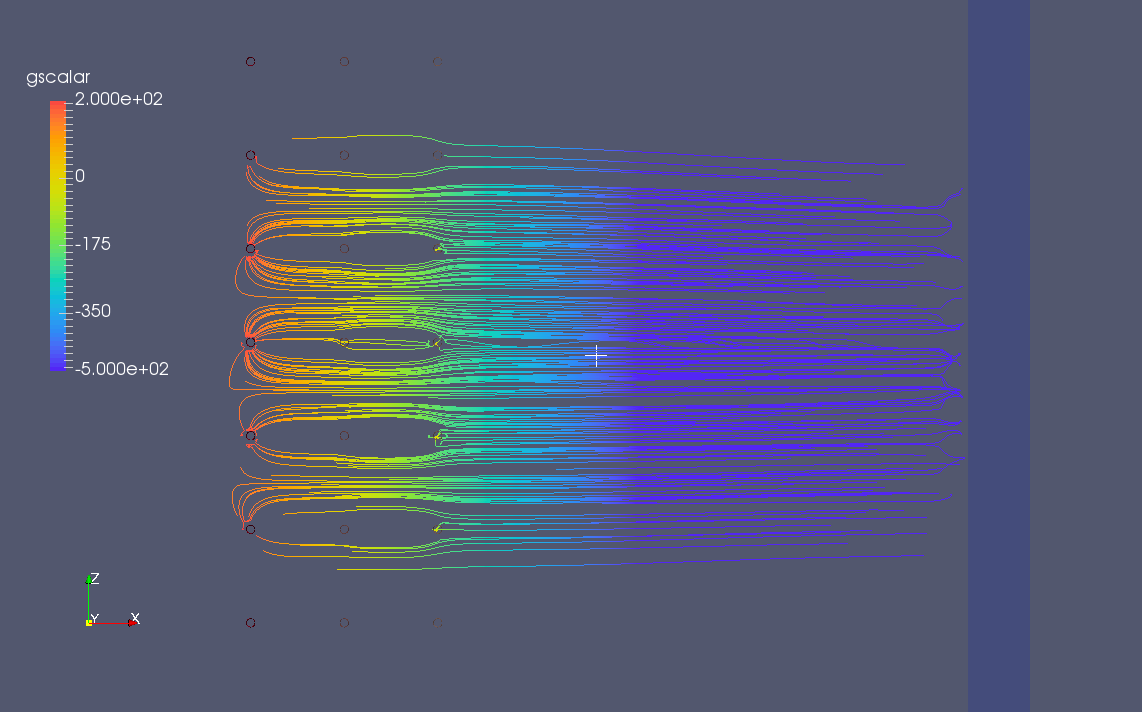
\includegraphics[width=\textwidth]{twodee-fine-steps-plan-gradfixed.png}      
    \end{column}
    \begin{column}{0.5\textwidth}
      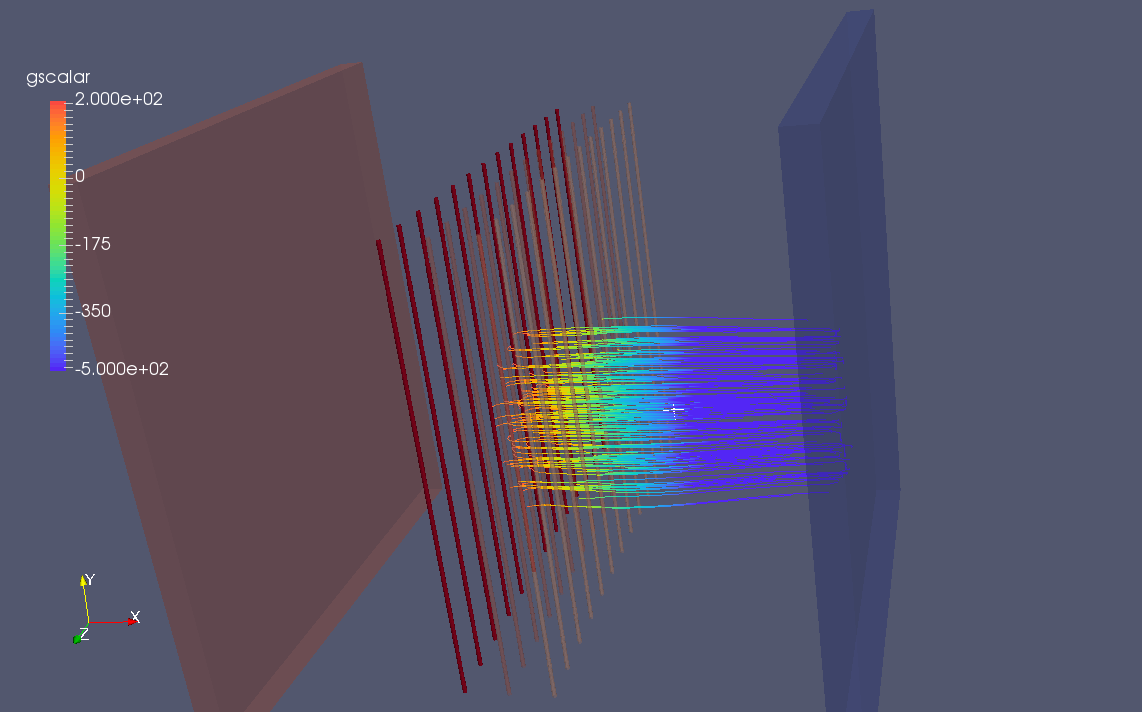
\includegraphics[width=\textwidth]{twodee-fine-steps-side-gradfixed.png}      
    \end{column}
  \end{columns}
  \footnotesize
  \begin{itemize}
  \item The steps no longer go wild in vertical direction.
  \end{itemize}

  \vfill

  Feel things are okay enough to move on to real 3D.
\end{frame}

\section{Caged Geometry}


\begin{frame}
  \frametitle{Caged Geometry Overview}

  New geometry features:
  \begin{itemize}
  \item Planar (instead of finite thickness) cathode.
  \item No ``ground plane'' (since there isn't one!)
  \item Wrap volume in mini ``field cage''.
  \item Bounded, fully filled wire planes.
  \end{itemize}

  \vfill

  Motivation for changes:
  \begin{itemize}
  \item Generically more realistic.
  \item Cage should make field more uniform.
  \item Better use of precious expensive $N^2$ triangles.
    \begin{itemize}\scriptsize
    \item Get rid of useless back side of cathode, ground plane
    \end{itemize}
  \item Add more wires in anticipation of Xin's requirements
  \item Can maybe use it look at detector edge effects.
  \end{itemize}
\end{frame}

\begin{frame}
  \begin{columns}
    \begin{column}{0.5\textwidth}
      \includegraphics[width=\textwidth]{caged-x.pdf}

      \includegraphics[width=\textwidth]{caged-z.pdf}
    \end{column}
    \begin{column}{0.5\textwidth}
      \includegraphics[width=\textwidth]{caged-iso.pdf}

      \includegraphics[width=\textwidth]{caged-y.pdf}
    \end{column}
  \end{columns}
\end{frame}
\begin{frame}
  \frametitle{Caged Surface Potentials}
  \begin{columns}
    \begin{column}{0.5\textwidth}
      \begin{center}
        \includegraphics[width=\textwidth]{caged-potential-back.png}

        \scriptsize Looking from behind wire plane.
      \end{center}
    \end{column}
    \begin{column}{0.5\textwidth}
      \begin{center}
        \includegraphics[width=\textwidth]{caged-potential-front.png}

        \scriptsize Looking through transparent cathode.
      \end{center}
    \end{column}
  \end{columns}
  
  \begin{center}
      500 V/cm over 30 cm (V-plane at 0 cm)
  \end{center}

  \scriptsize
  \begin{itemize}
  \item[$\rightarrow$] To check: problems with overlapping wires/cage?
  \end{itemize}

\end{frame}

\section{Next Steps}
\begin{frame}
  \frametitle{Next Steps}
  
  Caged:
  \begin{itemize}
  \item[1] Wait for field calculation jobs to finish and validate.
  \item[2] Step through field to generate instantaneous currents:
    \begin{itemize}
    \item Focus on on central wire from U, V, W planes.
    \item Start steps across entire $X=20-\epsilon$ plane
    \item Look steps staying away from cage.
    \item Collect steps in U/V/W wire ``region'' for average response
      \begin{itemize}
      \item And look at response as function of run along wire.
      \end{itemize}
    \item Etc for steps 1, 2, 3, ... wires over.
    \item Give to Xin family of wire vs. time waveforms to apply on data.
    \end{itemize}
  \end{itemize}
  Etc:
  \begin{itemize}
  \item Wrap up some presentation materials for Leon to present at uB meeting.
  \end{itemize}

\end{frame}

\begin{frame}
  \frametitle{Computing Limitiations}
  Problems:
  \begin{itemize}\footnotesize
  \item Need to increase precision 
    \begin{itemize}\scriptsize
    \item[$\rightarrow$] Just $\times 2 \Rightarrow$ couple hours for each field, may need $\times 4+$
    \item Gaussian quadrature order.
    \item Number and size of triangles.
    \item Spatial sampling resolution.
    \end{itemize}
  \item Resolution of spatial sampling also limited by system memory.
  \end{itemize}
  Possible solutions:
  \begin{itemize}\footnotesize
  \item Time/precision trade-off tuning
    \begin{itemize}\scriptsize
    \item[$\rightarrow$] but this also takes a long time.
    \end{itemize}
  \item Smarter spatial sampling - needed for larger volumes.
    \begin{itemize}\scriptsize
    \item Batch+stich spatial sampling, spread over more nodes.
    \item Non-uniform sampling, more densely near boundaries.
    \item[$\rightarrow$] requires fresh development, breaks code assumptions
    \end{itemize}
  \item Exploit more computers
    \begin{itemize}\scriptsize
    \item RACF requires non-trivial software install, running
      monopolizes entire node (but those 16 cores and 24GB RAM per
      node will be put to use!)
    \item Install Condor on 3rd floor workstations?
    \end{itemize}
  \end{itemize}
\end{frame}

\end{document}